

%\documentclass[letterpaper, 10 pt, conference]{ieeeconf}  % Comment this line out if you need a4paper

\documentclass[a4paper, 10pt, conference]{ieeeconf}      % Use this line for a4 paper

\IEEEoverridecommandlockouts                              % This command is only needed if 
                                                          % you want to use the \thanks command

\overrideIEEEmargins                                      % Needed to meet printer requirements.

% See the \addtolength command later in the file to balance the column lengths
% on the last page of the document

% The following packages can be found on http:\\www.ctan.org
%\usepackage{graphics} % for pdf, bitmapped graphics files
%\usepackage{epsfig} % for postscript graphics files
%\usepackage{mathptmx} % assumes new font selection scheme installed
%\usepackage{times} % assumes new font selection scheme installed
%\usepackage{amsmath} % assumes amsmath package installed
%\usepackage{amssymb}  % assumes amsmath package installed
\usepackage{graphicx} 
\usepackage{amsmath}
\usepackage{bm}
\usepackage{leftidx}
\usepackage{hhline}
\usepackage{multirow}
\usepackage{epstopdf}
\usepackage{subcaption}

\usepackage{caption}
\usepackage{lipsum}
\usepackage{mwe}
\usepackage{booktabs} 


\usepackage[noadjust]{cite}
\title{\LARGE \bf
Depth Enhanced Visual Odometry Based on \\ 
 Multi-State Constraint Kalman Filter
}


\author{Fumin Pang and Tianmiao Wang, \emph Member, \emph {IEEE}% <-this % stops a space
%\thanks{}% <-this % stops a space
\thanks{Fumin Pang and Tianmiao Wang are with the School of Mechanical Engineering and
	Automation, Beihang University, Beijing, 100191 China.
        {E-mail: fuminpang@buaa.edu.cn, itm@buaa.edu.cn}}%
}


\begin{document}



\maketitle
\thispagestyle{empty}
\pagestyle{empty}


%%%%%%%%%%%%%%%%%%%%%%%%%%%%%%%%%%%%%%%%%%%%%%%%%%%%%%%%%%%%%%%%%%%%%%%%%%%%%%%%
\begin{abstract}

There have been increasing demands for developing robotic system combining camera and inertial measurement unit in navigation task, due to their low-cost, lightweight and complementary properties. In this paper, we present a Visual Inertial Odometry(VIO) system which can utilize sparse depth to estimate 6D pose in GPS-denied and unstructured environments. The system is based on Multi-State Constraint Kalman Filter(MSCKF), which benefits from low computation load when compared to optimization-based method, especially on resource-constraint platform. Depth information offers real-metric perception of surroundings, and the combination of features w either with depth or  without depth gives a  more robust scale initialization and  higher  precision of the visual-inertial system. In this paper, we enhance the features with depth information to form  3D landmark position measurements in space, which reduces uncertainty  of position estimate. And we derivate measurement model to access compatibility with both 2D and 3D measurements.  In experiments, we  evaluate the performance of the system in different in-flight scenarios, both  cluttered room and  industry environment. The results suggest that the estimator is consistent, substantially improves the accuracy compared with original monocular-based MSKCF(mono-MSCKF) and achieves competitive accuracy with other research.




\end{abstract}


%%%%%%%%%%%%%%%%%%%%%%%%%%%%%%%%%%%%%%%%%%%%%%%%%%%%%%%%%%%%%%%%%%%%%%%%%%%%%%%%
\section{INTRODUCTION}


Accurate 6D pose estimate in unknown environment from a set of sensor measurements is one of the critical problems in robotics navigation task. Combination of complementary information from visual and inertial sensors is ubiquitous in mobile robot application with the requirement of high dynamic operation. Inertial sensors readings can be used to compute relatively accurate 6D pose iteratively in short period and give a real-metric estimate for absolute scale\cite{weiss2011real}. While visual sensor with the ability to provide rich texture of environment and bearing measurements for salient landmarks make it an efficient exteroceptive sensor to correct the motion and structure prediction. Each visual feature can always be tracked by a camera from a sequence of consecutive poses, which provide multiple constraint of camera motion and landmarks. Compared to another pose estimate paradigm Simultaneous Localization and Mapping (SLAM) which builds incremental map simultaneously, VIO pays more focus on efficient 6D pose estimate. This method has a long history and has achieved success in navigating Micro Aerial Vehicles(MAV) and cars. 
\begin{figure}[thpb]
	\centering
	
	\includegraphics[scale=0.37]{sparse2.jpg}
	
	\caption{(a) Features tracked at an image frame. The blue dots represent
		features whose depth comes from stereo matches. and the red dots represent features without
		depth. The proposed method uses both types of features in estimating 
		6D pose. (b) A disparity map from stereo  a corresponding to (a), which shows depth information is  only available in the vicinity of the camera. (c) A local  pointcloud built from (b),   colors encode distance. This local map shows the sparse nature for space landmarks.  }
	\label{figurelabel}
\end{figure}


To date, the majority of algorithms proposed for real-time VIO can be classified into two categories: extended Kalman filter-based methods and methods utilizing optimization approach. Filter-based approaches are the earlier ones used to solve SLAM and VIO problems. Davison et al. proposed one of the first real-time 3D monocular SLAM framework based on EKF in computer vision\cite{davison2007monoslam}. Based on this work, Roussillon et al. used IMU as a interoceptive to propagate position, orientation and velocity of platform in high dynamic environment\cite{roussillon2012high}. Jones and Soatto\cite{jones2011visual} built a EKF using Lie derivatives and studied observability in visual-inertial system, and the first time the analysis included the effects of unknown gravity and IMU-camera calibration parameters. Their results showed that the IMU biases, 3D velocity, absolute roll and pitch angles and IMU-camera transformation are observable. Some Similar conclusions were also drawn by  Kelly  et al.\cite{kelly2008combined}.


Meanwhile, optimization-based methods generally attain higher accuracy, as they re-linearize at each iteration to better deal with their nonlinear measurement models.
Leutenegger et al. describe a tightly coupled approach in which the robot poses and sparse 3D landmarks are estimated through minimize  a joint optimization problem using inertial error terms as well as the reprojection error of the landmarks in stereo image\cite{leutenegger2015keyframe}. Recently, a number of approaches have been proposed that directly use surface texture instead of visual features. Forster et al. propose a sparse direct methods approach in which IMU reading are pre-integrated as graph factors\cite{forster2015imu}. However, these methods always implement bundle adjustment in a sliding window of states, using multiple iterations to minimize cost function, which results in increased computational cost. Thus, filter-based methods might be a better choice for long-time running tasks, especially in resource constrained systems, such as micro aerial vehicles and Augmented Reality (AR) devices\cite{li2014visual}.

Multi-State Constraint Kalman Filter improve efficiency of filter-based method further\cite{mourikis2007multi}. Instead of including the 3D feature position in the state vector of the EKF, MSCKF maintains a sliding window of historical poses in state vector. The landmarks positions are triangulated from multiple observations form different camera poses when they slip away from field of view. Because the number of poses in sliding window is usually much less than the number of features, the computational complexity is reduced. Li et al. correct the observation properties of original MSCKF using First-Estimate Jacobian (FEJ)\cite{li2013high}. 

In this paper, we propose a method that can utilize sparse depth information along with the imagery based on MSCKF, inspired by \cite{zhang2014real} in which features with depth are combined with ones without depth to estimate poses via optimization method. The sparsity of depth is mainly reflected in two aspects. First, with limitation of the sensors, scenarios with large depth variation leave large area in the images where depth is unavailable spatially. Second, as in MSCKF paradigm, there need to exist multiple measurements for one feature from a series of different robot poses before its 3D position is triangulated. However, only a subset  of measurements for one feature has corresponding depth information temporally in general. The inevitable sparsity disenbles people to use ICP-like method in large scale environment to estimate posese. In this work, we fuse features with or without depth together to estimate the landmark position in space. We utilize 2D visual feature and depth to form a 3D measurement of a landmark. In the update step of this depth enhanced MSCKF, reprojection measurement errors for landmarks where depth is unavailable and 3D position measurement errors are jointed to correct the pose estimate. Here, we summary the contributions of this work:
  
\begin{itemize}
	\item {We propose a  MSCKF-based method  utilizing even sparse depth information to make up 3D measurements to  landmark positions, which reduces uncertainty of perception. Measurement model is adapted to be compatible with both 2D and 3D measurements  }
	
	\item {The proposed method has been tested on real-world data. The results demonstrate a lower drift than mono-MSCKF. The attained accuracy is  competitive with other research in this field. And the accuracy is also  verified by using the system in a mapping task.}
\end{itemize}

In this work, we use stereo camera to abtain depth information with consideration of weight and cost feasibility in MAV. But the proposed method is not limited to stereo cameras. It can be extended and adapted to various types of cameras as long as depth information can be acquired and associated.




\section{ESTIMATOR DESCRIPTION}

 Four different coordinate frames are used throughout
 the paper: we affix  camera-IMU rig body frame $\left\lbrace B \right\rbrace$ to IMU, to track the 6D motion with respect to a global coordinate frame, $\left\lbrace G \right\rbrace$. The camera coordinate frame, $  \emph CAM0 $, is $\left\lbrace C^0 \right\rbrace$. In this paper, it is $\emph CAM0 $ where features are tracked. An addtional camera , $  \emph CAM1 $, is added to form a stereo rig to estimate depth by potentially matching with features in $\emph CAM0 $. Its coordinate frame is $\left\lbrace C^1 \right\rbrace$.




\subsection{Overall Filter Structure and State Parametrization}
The full  state representation can be partitioned into two parts according to MSCKF paradigm. The first is the evolving current body state. As we affix body frame $\left\lbrace B \right\rbrace$ to IMU, we use $ \textbf x_{I}  $ to present body state. The body state at time \emph k is a 17-dimensional vector as follow:

\begin {equation}
\textbf x_{I,k} :=\left[  {\leftidx{_G^B}{\bar{\textbf q}}_k}^{ T} \ \
{\leftidx{^G}{\textbf p}_{B,k}}^T \ \
{\leftidx{^G}{\textbf v}_{B,k}}^T \ \
\textbf b_{g,k}^T \ \
\textbf b_{a,k}^T \ \ 
 t_{d,k}
\right]^T 
\end{equation}
In this world-centric presentation ,  $  {\leftidx{_G^B}{\bar{\textbf q}}_k}  $ is the unit quaternion representing the rotation which roatate vectors 
from the global frame  $\left\lbrace G \right\rbrace$ to the body frame  $\left\lbrace B \right\rbrace$. In this paper, all quaternions follow JPL convention \cite{sola2012quaternion}. $ {\leftidx{^G}{\textbf p}_{B,k}} $ is the vector from the
origin of $\left\lbrace G \right\rbrace$ to the origin of $\left\lbrace B \right\rbrace$ expressed in $\left\lbrace G \right\rbrace$ (i.e., the position of body in the global frame). $ {\leftidx{^G}{\textbf v}_{B,k}} $ is the vecotr repersenting original velocity of  frame  $\left\lbrace B \right\rbrace$ expressed in  $\left\lbrace G \right\rbrace$. $ \textbf b_{g,k} $ is the
bias on the gyro measurements $  \bm{ \omega}_m  $, $ \textbf  b_{a,k} $ is the bias on the
velocity measurements $ \textbf a_m $. $t_d$ is a scalar
modelling the unknown $ time \: offset$ between IMU and cameras and stays consitent. In this paper, we assume CAM0 and the depth sensor are synchronized temorally.

The second part of the full state is a sliding window of \emph N past body states, in which active feature tracks were visible. The \emph {i-th }body state, $ i = 0...N-1 $, inlcuding 6D pose and velocity, is a 10-dimensional vector. 
 
\begin {equation}
\textbf x_{B_i,k} :=\left[  {\leftidx{_{G}^{B_i}}{\bar{\textbf q}}_k}^{ T} \ \
{\leftidx{^B}{\textbf p}_{B_i,k}}^T \ \
{\leftidx{^G}{\textbf v}_{B_i,k}}^T
\right]^T
\end{equation}


Combining this two parts, the full state of MSCKF is a (17 + 10* \emph N)  vector consisting of  current body state estimate and \emph N last body states at time $  \emph k $. 

In MSCKF,  $ \emph Error \, State \, Kalman \, Filter$(ESKF)\cite{trawny2005indirect} is used to avoiding singularity brought by quaternions which use 4 dimensions to describe 3 degrees of freedom. While the error $ \left( \tilde x \right) $ between the true value $ \left(  x \right) $ and the estimated value $ \left( \hat x \right) $ for position, velocity , bias and $ t_d $ can be defined as $ \tilde x  = x - \bar x $  trivially, the error for quaternion is defined as:

\begin {equation}
\bm { \delta {\bar q}} := \bm{\hat{\bar q}}^{-1} \otimes \bm {  {\bar q}} \approx \left[\frac{1}{2}{ \bm {\delta \theta}}^T  \ \ 1\right]^T
\end{equation}
Using $  \bm {\delta \theta} $ to represent orientations
in the Kalman filter reduces their dimensionality to 3. As a result, the $\emph {error state} $ of the estimator  at time \emph k:

\begin {equation}
\tilde {\textbf x}_k :=\left[  {{\tilde{\textbf x}}_{I,k}}^{ T} \ \
{{\tilde{\textbf x}}_{B_0,k}}^{ T}  \ \
\ldots \ \
{{\tilde{\textbf x}}_{B_{N-1},k}}^{ T}  \ \
\right]^T
\end{equation}
where
\begin {equation}
\tilde{\textbf x}_{I,k} :=\left[  \leftidx{_B^G} { \bm {\delta \theta}}_{I}^T \ \
{\leftidx{^G}{\tilde {\textbf p}}_{B,k}}^T \ \
{\leftidx{^G}{\tilde {\textbf v}}_{B,k}}^T \ \
\tilde {\textbf  b}_{g,k}^T\ \
\tilde {\textbf b}_{a,k}^T \ \ 
\tilde {b}_{a,k}
\right]^T
\end{equation}
\begin {equation}
\tilde{\textbf x}_{B_i,k} :=\left[  \leftidx{_{B_i}^G} { \bm {\delta \theta}}_{I}^T \ \
{\leftidx{^G}{\tilde {\textbf p}}_{B_i,k}}^T \ \
{\leftidx{^G}{\tilde {\textbf v}}_{B_i,k}}^T \ \
\right]^T
\end{equation}


The full error state has  (16 + 9 \emph N) dimensions. Accordingly, the MSCKF error state covariance $ \bm{P} $ is a (16 + 9 \emph N) $ \times $ (16 + 9 \emph N) matrix. 



\subsection{Filter Propagation}

Every time an IMU measurement is received,
it is used to propagate the IMU state. As mentioned before, IMU measurement provide rotational velocity $ \bm {\omega}_m $ and $ \bm a_m $, described as below equations: 
\begin{equation}
\bm{\omega}_m ={\leftidx{^G}{ {\bm \omega}}_{}} + \bm b_g + \bm n_g
\end{equation}
\begin{equation}
\bm{a}_m =   \leftidx{_G^B}{{\textbf R}}  \left( \leftidx{^G}{\bm a} - \leftidx{^G}{\bm g}\right) + \bm b_a +\bm n_a
\end{equation}
where $ \leftidx{_G^B}{{\textbf R}} $ is the rotation matrix cooresponding to $  \leftidx{_G^I}{{\textbf q}} $. $\leftidx{^G}{\bm g}  $ is the gravitational acceleration.  $ \bm n_g $ and $ \bm n_a $  are zero-mean white Gaussian noise vectors. Using these measurements, we can
write the dynamics of the filter state vector as:
\begin{equation}
\leftidx{_G^I}{\dot {\bar{\textbf q}}}(t)=\frac{1}{2} \bm \Omega\left(  {\bm \omega}_m (t)-\bm b_g(t) - \bm n_g(t) \right)\leftidx{_G^I}{ {\bar{\textbf q}}} 
\end{equation}
\begin{equation}
{\leftidx{^G}{\dot {\textbf v}}_{B}}(t)=\leftidx{_G^B}{{\textbf R}}^T(t)\left( \bm a_m(t)-\bm b_a(t)-\bm n_a(t) \right)+  \leftidx{^G}{\bm g}
\end{equation}
\begin{equation}
{\leftidx{^G}{\dot {\textbf p}}_{B}}(t)= {\leftidx{^G}{ {\textbf v}}_{B}}(t)
\end{equation}
\begin{eqnarray}
{ \bm {\dot b_g}}(t) =  \bm n_{wg}(t) & { \bm {\dot b_a}}(t) =  \bm n_{wa}(t)
\end{eqnarray}
\begin{equation}
{{\dot {t}_d}}(t)= 0
\end{equation}
where $ \bm \Omega $ is the quaternion multiplication matrix corresponding to the angular velocity vector $ \bm \omega $. The fourth line models the biases  as random walk processes wiht noises $  \bm n_{wg} $ and $ \bm n_{wa} $. In this work, we consider the time offset,$ t_d $, is not changing temporally. We follow the approach described in \cite{li2013high} for propagating the state estimates in a discrete-time implementation. Further, a fifth-order
Runge-Kutta procedure is used for propagate quaternion.  Besides the current body state, all  states in sliding window   remain unchanged during propagation.



 Linearized continuous-time model of  current state error state, $ {{\tilde{\textbf x}}_{I}} $, can be drawn from ($9$)-($13$):
\begin{equation}
{\dot{\tilde{\textbf x}}_{I}} =  \bm F{\tilde{\textbf x}}_{I}+\bm G \bm n_I
\end{equation}
where $ \bm F $ is the continuous-time error-state transition matrix. $ \bm G $ is 
the Jacobian of current body error state with respect to the noise vector  $ \bm n_I = [\bm n_g^T \ \bm n_{a}^T \  \bm n_{wg}^T \ \bm n_{wa}^T]^T $. 


\begin{figure}[thpb]
	\centering
	
	\includegraphics[scale=0.4]{trian1.jpg}
	
	\caption{ 3D measurement can be achieved by fusing two visual measurements from stereo camera. Mean of 3D measurement can be calculate from triangulation, and the covariance $ \Sigma_p $ comes from merging two 3D Gaussian distributions, $ \Sigma_{p_0} $ and $ \Sigma_{p_1} $. This Bayesian fusion results in smaller 3D uncertainty than either $ \Sigma_{p_0} $ or $ \Sigma_{p_1} $, visualized as a smaller  ellipsoid.  The pixel bearing vector uncertainty involve visual feature uncertainty and scale.}
	\label{figurelabel}
\end{figure}

In addition, state covariance matrix is also propagated accordingly:

\begin{equation}
\bm{P}(t_{k+1})= \left[  \begin{matrix} 
 \bm {\Phi}_{I_k}\bm{P_{II}}(t_{k}) \bm {\Phi}_{I_k}^T + \bm {Q_d}  & 
\bm {\Phi}_{I_k}\bm{P_{IB}}(t_{k}) \\
\bm{P_{IB}}^T(t_k) \bm {\Phi}_{I_k}^T & 
\bm{P_{BB}}(t_k)  \\
\end{matrix}   \right] 
\end{equation}
where $ \bm {\Phi}_{I_k} $ is the discrete-time error-state transition matrix at \emph k, linearization of  $ \bm F $, computed in closed form as shown in \cite{li2013high}. $ \bm {Q_d}  $ is discrete-time IMU noise matrix, and $ \bm{P_{II}} $,$ \bm{P_{BB}} $, and
$ \bm{P_{IB}} $ are the partitions of the filter covariance matrix for
the current body state, the past body states, and the cross-terms between
them, respectively.




\subsection{State Augmentation}
Upon recording a new image, a copy of current body rotation, position and velocity is appended
to the state vector, and the covariance matrix of the MSCKF is augmented accordingly.


\subsection{Mean and Covariance of 3D measurement}

In this paper, visual measures from stereo camera form a 3D measurement of a landmark  when the depth is available. Stereo measuremnt can efficiently reduce the uncertainty (covariance) of 3D position esttmate . We consider one feature,$ \bm f $, which is observed  by  stereo rig at timestep $ \bm {   i }$. We will derivate its mean and covariance of 3D position measurement. 

First, in frame $\left\lbrace C^0 \right\rbrace$, landmark position $ \leftidx{^{C_i^0}}{ { \bm p}}_f  = [  \leftidx{^{C_i^0}}{  X} \; \leftidx{^{C_i^0}}{  Y} \; \leftidx{^{C_i^0}}{  Z} ]^T$  is calculated by stereo triangulation. We present its 3D measurment  using a pixel bearing vector $ [  \alpha \;  \beta ]^T $ and a inverse depth scalar $  \rho $ :

\begin{equation}
\leftidx{^{C_i^0}}{ {\bm { z}}}_3 = \left[ \begin{matrix}  
\leftidx{^{C_i^0}}{ { \alpha}} \\
\leftidx{^{C_i^0}}{ { \beta}} \\
\leftidx{^{C_i^0}}{ { \rho}}
 \end{matrix}\right]  = \bm \pi_3\left(  \begin{matrix}  
 \leftidx{^{C_i^0}}{ { X}} \\
 \leftidx{^{C_i^0}}{ { Y}} \\
 \leftidx{^{C_i^0}}{ { Z}}
 \end{matrix} \right) = \left[ \begin{matrix}  
 \frac{\leftidx{^{C_i^0}}{ {  X}}^{}}{\leftidx{^{C_i^0}}{ {  Z}}^{}}\\
 \frac{\leftidx{^{C_i^0}}{ { Y}}^{}}{\leftidx{^{C_i^0}}{ {   Z}}^{}}\\
 \frac{1}{\leftidx{^{C_i^0}}{ { Z}}^{}}\\
 \end{matrix}\right] 
\end{equation}
\begin{figure}[thpb]
	\centering
	
	\includegraphics[scale=0.26]{multi1.eps}
	
	\caption{ An example indicates one feature $ f_j $ observed by camera at 4 pose. At $ T_1 $ and $ T_3 $, depth is availible which generates 3D measurements, while  at $T_2$ and $T_4$, no matches can be found in $ CAM1 $ resulting in two 2D measurements. Landmark position cooresponding to $ f_j $ is estimated by minimizing either 2d or 3D measurement errors through least-square method.   }
	\label{figurelabel}
\end{figure}

Similarly, in $\left\lbrace C_1 \right\rbrace$, the 3D measurement $ \leftidx{^{C_i^1}}{\bm { z}}_3 $ of $\leftidx{^{C^0}}{\bm  { p}}_f  $ is 

\begin{equation}
\leftidx{^{C_i^1}}{\bm { z}}_3 = \left[ \begin{matrix}  
\leftidx{^{C_i^1}}{ \alpha} \\
\leftidx{^{C_i^1}}{ \beta} \\
\leftidx{^{C_i^1}}{ \rho}
\end{matrix}\right]  = \bm \pi_3\left( \leftidx{^{C^1}_{C^0}}{\bm R}\left(  \begin{matrix}  
\leftidx{^{C_i^0}}{ X} \\
\leftidx{^{C_i^0}}{ Y} \\
\leftidx{^{C_i^0}}{ Z} 
\end{matrix} \right) + \leftidx{^{C^1}}{\bm p}_{C^0}
 \right)
\end{equation}
As above, $\bm  \alpha$, $\bm  \beta$ are given  by pixel coordinates in image with measurement noise $\bm {diag}({  \sigma}_{\alpha}^2, { \sigma}_{\beta}^2 )  $. $  \rho $ can be calculated by inversing depth. Following paper, we assume $  \rho \sim  {\mathcal N}\left(  \rho , { \sigma}_{\rho}^2 \right) $, where ${ \sigma}_{\rho}$ is set manually.


From (16)-(17), the covariance of  Gaussian distribution in Euclidean space of $\leftidx{^{C^0}}{\bm { p}}_f $ can be fused by the two measurements uncertainties:


\begin{equation}
{\bm \Sigma}_{p^j} = {\bm J_{p^j}}{\bm {diag}\left( {  \sigma}_{\alpha^j}^2, { \sigma}_{\beta^j}^2,{ \sigma}_{\rho^j}^2 \right) } {\bm J_{p^j}}^T
\end{equation}
where $ j = 0,1 $ and $
\bm J_{p^j}= \frac{\partial{\leftidx{^{C^0}}{\bm { p}}_f}}{\partial{\leftidx{^{C_i^j}}{\bm { z}}_3 }}
$.

Given two 3D measurement covariances $ {\bm \Sigma}_{p^0}  $ and $ {\bm { \Sigma}}_{p^1} $ , we can fuse  the position covariance using a  Bayesian update step \cite{stroupe2001merging}:
 
\begin{equation}
\leftidx{^{C_{i}}}{\bm { \Sigma}}_{p} ={\bm { \Sigma}}_{p^0}\left(  {\bm { \Sigma}}_{p^0} + {\bm { \Sigma}}_{p^1}\right)^{-1} {\bm { \Sigma}}_{p^1}
\end{equation}
Fusing two 3-dimensional Gaussian distributions  reduces the uncertainty 
of the distribution (see Fig.2). Finally, the 3D measurement mean and  covariance can be derivated:

\begin{eqnarray}
\leftidx{^{C_{i}}}{ {\bm { z}}}_3 = \left[ \begin{matrix}  
\leftidx{^{C_{i}}}{ { \alpha}} \\
\leftidx{^{C_{i}}}{ { \beta}} \\
\leftidx{^{C_{i}}}{ { \rho}}
\end{matrix}\right] &&
\leftidx{^{C_i}}{\bm { \Sigma}_3} = {\bm J_{\bm \pi_3}} \leftidx{^{C_{i}}}{\bm { \Sigma}}_{p}{\bm J_{\bm \pi_3}}^T
\end{eqnarray}
where ${\bm J_{\bm \pi_3}} = \frac{\partial{\leftidx{^{C_{0,i}}}{\bm { z}}_3 }}{\partial{\leftidx{^{C_0}}{\bm { p}}_f}} $. The 3D covariance in Euclidean space is transformed to bearing and inverse depth parameterization space. Here,  for simplicity,  $ C_i $ is used to present camera frame $C_i^0 $ at timestep $ \emph i$.  Thus, fusing the visual measures in stereo provides a more precise  estimate on landmark position and reduces uncertainty by fusing the two Gaussian distributions, which will potentially improve performance of viual odometry accuracy. 


\subsection{Depth Enhanced Feature Position Estimation}

In this work, once a tracked feature is lost in current frame,  $  \emph {CAM0} $, the corresponding landmark position need to be estimated. Compared to original MSCKF which uses triangultion from a sliding window of 2D  imagery measeurements, we  utilize both  2D and  3D measures.

To describe the position estimate process and update model, we consider one landmard,$  \leftidx{^G}{\bm p}_{f_j} $, which is observed at a set of poses, $\left\lbrace \bm T_i = \left\lbrace  \leftidx{^{C_i}_{G}}{\bm R}, \leftidx{^{G}}{\bm p}_{C_i} \right\rbrace \in SE(3)  \right\rbrace $ with $ i = 1,2,3,4 $ (see Fig.3). In $ C_1$ and $ C_3 $, depth is availible.We initialize the optimization by estimating the position of feature $ f_j$ in camera frame $ C_1$ using a linear least-squares method \cite{clement2015battle}. We can express the feature position in camera frame $ C_i$
in terms of its position in camera frame $ C_1$  as

\begin{equation}
\leftidx{^{C_i}}{\bm {\hat p}}_{f_j} = \leftidx{^{C_i}_{C_1}}{\bm {\hat R}}\leftidx{^{C_1}}{\bm {\hat p}}_{f_j} + \leftidx{^{C_i}}{\bm { \hat p}}_{C_1}
\end{equation}
we can write the 2D imagery measurement error as

\begin{equation}
\bm e_{2,i}(\leftidx{^{C_1}}{\bm {\hat p}}_{f_j})= \leftidx{^{C_i}}{{\bm z}_{2,i}} - \bm \pi_2 \left( \leftidx{^{C_i}_{C_1}}{\bm {\hat R}}\leftidx{^{C_1}}{\bm {\hat p}}_{f_j} + \leftidx{^{C_i}}{\bm {\hat p}}_{C_1}\right) 
\end{equation}
where $ \leftidx{^{C_i}}{{\bm z}_{2,i}}  $ is the pixel bearing vector given by feature coordinate and  
\begin{equation}
 \bm \pi_2(\bm h) = \left[ \begin{matrix}  
 \frac{h(1)}{h(3)}\\
 \frac{h(2)}{h(3)}

 \end{matrix} \right] 
\end{equation}
and 3D measurement error as
\begin{equation}
\bm e_{3,i}(\leftidx{^{C_1}}{\bm {\hat p}}_{f_j})=  \leftidx{^{C_i}}{{\bm z}_{3,i}}- \bm \pi_3 \left( \leftidx{^{C_i}_{C_1}}{\bm {\hat  R}}\leftidx{^{C_1}}{\bm {\hat p}}_{f_j} + \leftidx{^{C_i}}{\bm {\hat  p}}_{C_1}\right) 
\end{equation}

\begin{figure}[thpb]
	\centering
	
	\includegraphics[scale=0.6]{NumOfdepthEnhancedMeas.eps}
	
	\caption{Boxplot on simulation result about of 3-axis errors of $ {\bm { p}}_{f_j} $ presented in $ C_1 $, in which   different amount of 3D measurment is applied to estimate landmark position .   We generate 50 features within  a distance of 1-5 meters in front of cameras, and the  sliding window size is 15. All feature postions are estimated with 3D measuerment amounts varying from 1 to 15, respectively. The results indicate more 3D measurments reduce the measurments error, espacially along z-direction in local coordinate. }
	\label{figurelabel}
\end{figure}

By stacking the measurements together, the least-squares system then becomes
\begin{equation}
\left( \bm J^T \bm W^{-1} \bm J\right) \bm \delta \leftidx{^{C_1}}{\bm p}_{f_j}^{\star} = - \bm J^T \bm W^{-1} \bm e \left( \leftidx{^{C_1}}{\bm {\hat p}}_{f_j}\right) 
\end{equation}
where $\bm e \left( \leftidx{^{C_1}}{\bm {\hat p}}_{f_j}\right) $ is stacked vector of four measurement errors and  $\bm J $ is  stacked  matrix  of four  Jacobians of measurement error with respect to $\leftidx{^{C_1}}{\bm { \hat p}}_{f_j}$ and 
\begin{equation}
\bm W = \bm {diag}\left\lbrace \leftidx{^{C_1}}{\bm { \Sigma}_3} \ \ \leftidx{^{C_2}}{\bm { \Sigma}_2} \ \ \leftidx{^{C_3}}{\bm { \Sigma}_3} \ \ \leftidx{^{C_4}}{\bm { \Sigma}_2}  \right\rbrace 
\end{equation}
with $ \leftidx{^{C_i}}{\bm { \Sigma}_2} = \bm {diag} \left\lbrace  { \sigma}_{\alpha_i}^2, { \sigma}_{\beta_i}^2 \right\rbrace  $. $ \leftidx{^{C_i}}{\bm { \Sigma}_3}$ is calculated  in  previous section.
 
 
 
 
In practice, in order to improve numerical stability, inverse depth parameterization \cite{montiel2006unified} is used. After iterative optimization, we get $\leftidx{^{C_1}}{\bm { \hat p}}_{f_j}$ and further $\leftidx{^{G}}{\bm { \hat p}}_{f_j}$. A simulation on how  different  quantities of 3D measurements in sliding window effects accuracy of position estimate is showed in Fig.4. The result shows depth information can observably benefits the estimation, especially along z-axis in local coordinate .







\subsection{Depth Enhanced Filter Update}

Once the landmark position $\leftidx{^{G}}{\bm { \hat p}}_{f_j}$ is estimated, we can calculated the measurement residuals for either 2D measurments or 3D measurements  to update the system.

\begin{equation}
\bm {r}_i^{(j)} = \leftidx{^{C_i}}{{\bm z}_{i}^{(j)}} - \leftidx{^{C_i}}{{\bm {\hat z}}_{i}^{(j)}}
\end{equation}
where for 2D measuremnt, $ \bm {r}_i^{(j)} $ is $ 2 \times 1 $ and 
\begin{equation}
 \leftidx{^{C_i}}{{\bm {\hat z}}_{2,i}^{(j)}} = \bm \pi_2 \left( \leftidx{^{C_i}_{G}}{\bm {\hat  R}} \left( {\leftidx{^{G}}{\bm {\hat p} }_{f_j}}-{\leftidx{^{G}}{\bm {\hat p}}_{C_{i}}}  \right) \right) 
\end{equation}
and for 3D measurement, $ \bm {r}_i^{(j)} $ is $ 3 \times 1 $ and 
\begin{equation}
\leftidx{^{C_i}}{{\bm {\hat z}}_{3,i}^{(j)}} = \bm \pi_3 \left( \leftidx{^{C_i}_{G}}{\bm {\hat  R}} \left( {\leftidx{^{G}}{\bm {\hat p} }_{f_j}}-{\leftidx{^{G}}{\bm {\hat p}}_{C_{i}}}  \right) \right) 
\end{equation}



Linearizing about the estimates for the body pose and
for the feature position, the residual of  $ (24) $ can be approximated as:
\begin{equation}
\bm {r}_i^{(j)} =\bm{H_{x_{B_i}}^{(j)}}{\tilde {\bm x}}+\bm{H_{f_{i}}^{(j)}}{\leftidx{^{G}}{\bm {\tilde p}}_{f_{j}}}+{\bm n_i^{(j)}}
\end{equation}
where the matrices $ \bm{H_{x_{B_i}}^{(j)}} $ and $ \bm{H_{f_{i}}^{(j)}} $ are the corresponding Jacobians of the measurement $  \bm {\hat z}_{i}^{(j)} $ with respect to the state and the feature position, respectively, and $ {\leftidx{^{G}}{\bm {\tilde p}}_{f_{j}}} $ is the error in the
position estimate of $ \bm f_j $. $ \bm n_i^{(j)} $ is the  measurement noise with covariance either $ \leftidx{^{C_i}}{\bm { \Sigma}_2}$ or $ \leftidx{^{C_i}}{\bm { \Sigma}_3}$. $ \bm{H_{x_{B_i}}^{(j)}} $ and $ \bm{H_{f_{i}}^{(j)}} $ are given by

\begin{equation}
\bm{H_{x_{B_i}}^{(j)}}=\bm J_{\pi,i}^{(j)}\left[\begin{matrix} \bm 0_{3 \times 15} & \bm M_{t_d,i} & \bm 0_{3 \times 9(i-1)} & \bm M_{B_i} & \bm 0_{3 \times 9(N-l)}
\end{matrix} \right] 
\end{equation}

\begin{equation}
\bm{H_{f_i}^{(j)}}=\bm J_{\pi,i}^{(j)} \leftidx{_B^{C_0}}{ {\textbf R}} \leftidx{_G^B}{\hat {\textbf R}} \left( t + \hat t_d \right) 
\end{equation}
where
\begin{equation}
\bm M_{t_d,i}  = \leftidx{_B^{C_0}}{ \textbf R} \left( 
\lfloor
 \leftidx{_G^B}{\hat {\textbf R}} \left(  {\leftidx{^{G}}{\bm {\hat p} }_{f_j}}-{\leftidx{^{G}}{\bm {\hat p}}_{B_{i}}} 
  \right) \times
 \rfloor
 \leftidx{^B}{\bm \omega} -   \leftidx{_G^B}{\hat {\textbf R}} {\leftidx{^{G}}{\bm {\hat v}}_{B_{i}}} 
 \right) 
\end{equation}

\begin{equation}
\bm M_{B_i} =\leftidx{_B^{C_0}}{ {\textbf R}} \leftidx{_G^B}{\hat {\textbf R}} \left( t + \hat t_d \right) 
\left[\begin{matrix}
 \lfloor (\leftidx{^{G}}{\bm { p}}_{f_{j}}-\leftidx{^{G}}{\bm {\tilde p}}_B)\times \rfloor & 
 - \bm I_3 &
  \bm 0_3
\end{matrix} \right] 
\end{equation}
 $ \lfloor \bm c\times \rfloor  $ is the skew symmetric matrix corresponding to vector $ \bm  c $. And for more details,the nonzero blocks in $ \bm{H_{x_{B_i}}^{(j)}} $ are  the Jacobians with respect to  body rotation  and body position , respectively. $ \bm J_{\pi,i}^{(j)} $ is the Jacobian of the perspective model depending on 2D or 3D measurement type:
\begin{equation}
\bm J_{\pi_2,i}^{(j)}=  \frac{1}{\leftidx{^{C_{i}}}{\bm {\hat Z}}^{(j)}}\left[ \begin{matrix} \bm 1 & \bm 0 & - \dfrac{\leftidx{^{C_{i}}}{\bm {\hat X}}^{(j)}}{\leftidx{^{C_{i}}}{\bm {\hat Z}}^{(j)}} \\ \bm 0 & \bm 1 & - \dfrac{\leftidx{^{C_{i}}}{\bm {\hat Y}}^{(j)}}{\leftidx{^{C_{i}}}{\bm {\hat Z}}^{(j)}} \end{matrix} \right]
\end{equation}

\begin{equation}
\bm J_{\pi_3,i}^{(j)}=  \frac{1}{\leftidx{^{C_{i}}}{\bm {\hat Z}}^{(j)}}\left[ \begin{matrix} \bm 1 & \bm 0 & - \dfrac{\leftidx{^{C_{i}}}{\bm {\hat X}}^{(j)}}{\leftidx{^{C_{i}}}{\bm {\hat Z}}^{(j)}} \\
 \bm 0 & \bm 1 & - \dfrac{\leftidx{^{C_{i}}}{\bm {\hat Y}}^{(j)}}{\leftidx{^{C_{i}}}{\bm {\hat Z}}^{(j)}}  \\
 \bm 0 & \bm 0 & - \dfrac{1}{\leftidx{^{C_{i}}}{\bm {\hat Z}}^{(j)}} 
 
 \end{matrix} \right]
\end{equation}

Stacking the residuals
of all measurements either 2D or 3D , we can get:
\begin{equation}
\bm {r}^{(j)} =\bm{H_{x_{B}}^{(j)}}{\tilde {\bm x}}+\bm{H_{f}^{(j)}}{\leftidx{^{G}}{\bm {\tilde p}}_{f_{j}}}+{\bm n^{(j)}}
\end{equation}
where $ \bm {r}^{(j)} $, $ \bm{H_{x_{B}}^{(j)}} $, $ \bm{H_{f}^{(j)}} $, and $ {\bm n^{(j)}} $ are block vectors or matrices with elements $ {r}_i^{(j)} $ , $ \bm{H_{x_{B_i}}^{(j)}} $, $ \bm{H_{f_{i}}^{(j)}} $, and $ {\bm n_i^{(j)}} $. Eq.(37) can not be directly used for measurement update in MSCKF. Because the term $ {\leftidx{^{G}}{\bm {\tilde p}}_{f_{j}}} $ is not part of state vector. In order to transform (37) into a standard form for update, we can compute a semi-unitary matrix $ \bm A $ whose columns form
the basis of the left nullspace of $ \bm{H_{f}^{(j)}} $, and multiply both sides of (37) by $ \bm A $ \cite{mourikis2007multi} .

\begin{equation}
\begin{split}
\bm {r_o}^{(j)} = \bm A^T\bm {r}^{(j)} & =\bm A^T \bm{H_{x_{B}}^{(j)}}{\tilde {\bm x}}+\bm 0+ \bm A^T{\bm n^{(j)}} \\
& = \bm{H_{o}^{(j)}}{\tilde {\bm x}} + {\bm n_0^{(j)}}
\end{split}
\end{equation}

Now, we obtain the useful form for filter update. We assume the quantity of 2D measurments is $\mathcal M_2^{(j)}$, while $\mathcal M_3^{(j)}$ for 3D measurements. Thus $ \bm A $ has dimension $  (2 \mathcal  M_2^{(j)} + 3 \mathcal  M_3^{(j)} ) \times
(2 \mathcal  M_2^{(j)} + 3 \mathcal  M_3^{(j)} -3)  $ and  $ \bm {r_o}^{(j)}  $ has dimension $ (2 \mathcal  M_2^{(j)} + 3 \mathcal  M_3^{(j)} -3) \times 1 $. The
covariance matrix of $ {\bm n_o^{(j)}} $ is  $ \bm { \Sigma_o}^{(j)}  = \bm A^T{\bm \Sigma^{(j)}}\bm A $.
We can now stack all the errors $ \bm {r_o}^{(j)}  $ for all the features selected for update.
\begin{equation}
\bm {r_o}= \bm{H_o}{\tilde {\bm x}} + {\bm n_o}
\end{equation}

To reduce the
computational complexity of the MSCKF update, a QR-decomposition of $ \bm{H_o} $ is employed.
 
Finally, we calculate the Kalman gain. And the state vector and covariance are updated following the  description in \cite{mourikis2007multi}.

\section{IMPLEMENTATION DETAILS}
\subsection{Feature Detection and Match}
In this paper, We extracted 60-to-200 salient point features  using Oriented FAST and Rotated BRIEF (ORB) detector in each frame \cite{rublee2011orb}. ORB feature maintains a image pyramid to find the best cornors independent of the scale. For  compromise of precision and efficiency, we use a 3-level pyramid while the scale factor between adjacent levels is 1.2. The relationship between feature pixel bearing vector uncertainty and level in which this feature is detected is 

\begin{eqnarray}
\sigma_{\alpha} = \frac{\sigma_u}{f_u} \left(1.2 \right)^{level} &&
\sigma_{\beta} = \frac{\sigma_v}{f_v} \left(1.2 \right)^{level} 
\end{eqnarray}
 $ \sigma_u $   and ${\sigma_v}$ are  feature imagery coordinate isotropic uncertainties at 0-level image in pyramid. $f_u $ and  $f_v$ are camera focal length.
 
 Image is divide in cells of fixed size (e.g. $ 32 \times 30$ pixels). This results in evenly distributed features in image by limiting each cell only maintaining the strongest feature ,if it exists. 

Each feature track always trys to estimate 3D position of the cooresponding landmark in the  frame where  first detected. If stereo matching is availible (the case as shown in Fig.3) when feature is detected, the local landmark position is calculated by stereo triangulation. Otherwise, the local position will be estimated by first two visual measurements from $CAM0$. Like in stereo triangulation case, the local position uncertainty is also calculated. After this, 2D-to-3D matching can be achieved for the following images. Reprojecting the this 3D local point ,whcih  gives a good searching guess for  feature matches in succeeding images, keeps the algorithm efficient. 
\subsection{Outlier Detection}
After the local feature position is achieved when it is first detected, the position uncertianty is reprojected into succeeding images 
\begin{equation}
\leftidx{^{C_{cur}}}{\bm { S}} = {\bm J_{\bm h}} \leftidx{^{C_{first}}}{\bm { \Sigma}}_{p}{\bm J_{\bm h}}^T
\end{equation}
where $ {\bm J_{\bm h}}$ is the $ 2 \times 3$ Jacobian of $ \bm h( \bullet )$ which projects 3D points in the frame where the feature is first detected to current image with respect to the feature position. Than the $ 2\sigma$ uncertainty ellipse derivated from $ 2 \times2$ matrix $\leftidx{^{C_{cur}}}{\bm { S}} $  in image frame is  used to predict potential matching and reject outliers.


Further, once $\bm r_o^{(j)} $ and $\bm H_o^{(j)}$ are calculated in (38), we proceed to carry out a
Mahalanobis gating test for the residual $\bm r_o^{(j)}$.   Here a  95th percentile of the $ \chi^2 $ test with  $ (2 \mathcal  M_2^{(j)} + 3 \mathcal  M_3^{(j)} -3)  $ degrees of freedom is made.



\section{EXPERIMENTS}



\begin{figure}[thpb]
	\centering
	
	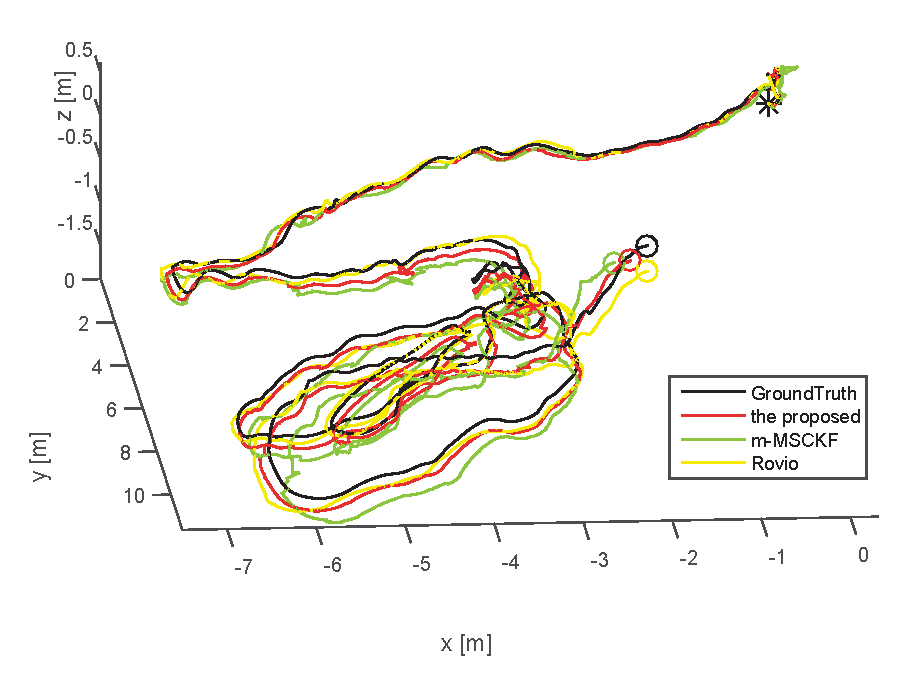
\includegraphics[scale=0.6]{MH01_3compare_legend.eps}
	
	\caption{Comparision on trajectory estimations of  mono-MSCKF, Rovio and our method on $MH\_01\_easy$ dataset. }
	\label{figurelabel}
\end{figure}
\begin{figure}[thpb]
	\centering
	
	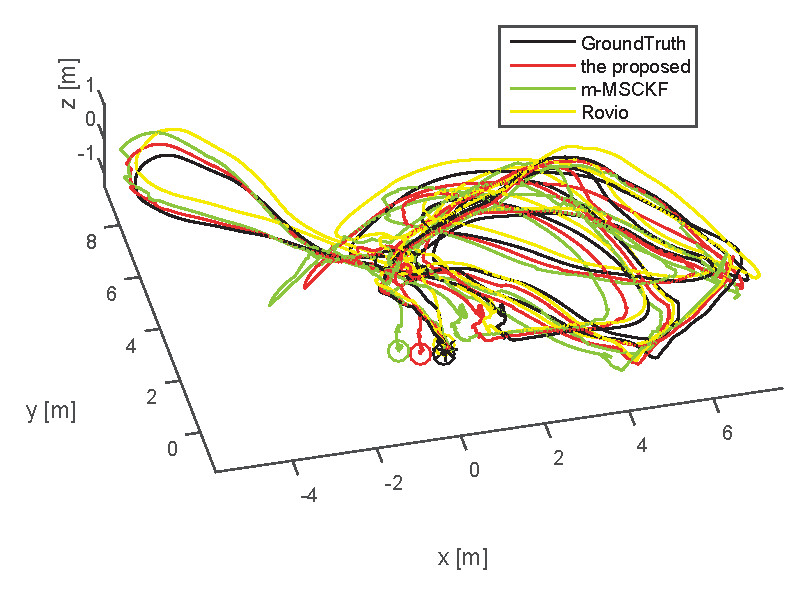
\includegraphics[scale=0.6]{MH03_3compare_legend.eps}
	
	\caption{Comparision on trajectory estimations of  mono-MSCKF, Rovio and our method on $MH\_03\_medium$ dataset. }
	\label{figurelabel}
\end{figure}
\begin{figure}[thpb]
	\centering
	
	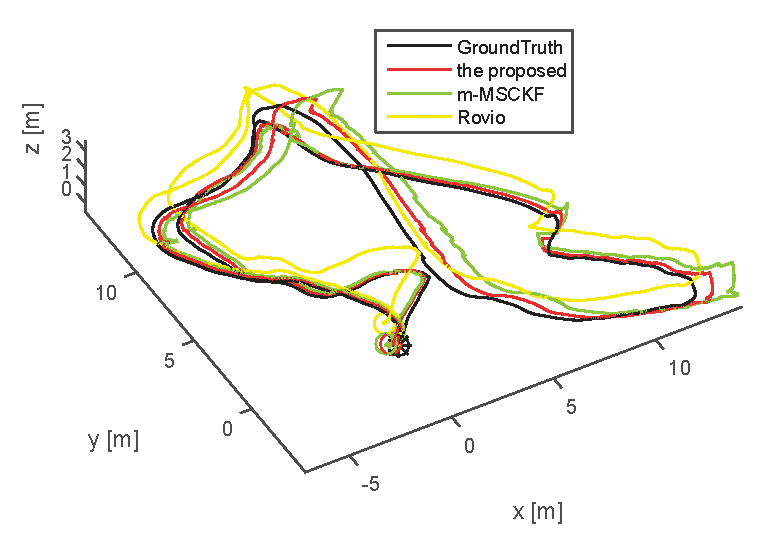
\includegraphics[scale=0.6]{MH05_3compare_legend.eps}
	
	\caption{Comparision on trajectory estimations of  mono-MSCKF, Rovio and our method on $MH\_05\_difficult$ dataset. }
	\label{figurelabel}
\end{figure}




\begin{table*} % Add the following just after the closing bracket on this line to specify a position for the table on the page: [h], [t], [b] or [p] - these mean: here, top, bottom and on a separate page, respectively
	\caption{ATE on EuRoC / ASL Dataset}
	\centering % Centers the table on the page, comment out to left-justify
	\begin{tabular}{p{2.2cm} | p{1.2cm} p{1.2cm} p{1.5cm} | p{1.2cm} p{1.2cm} p{1.5cm} | p{1.2cm} p{1.2cm} p{1.2cm}} % The final bracket specifies the number of columns in the table along with left and right borders which are specified using vertical bars (|); each column can be left, right or center-justified using l, r or c. To specify a precise width, use p{width}, e.g. p{5cm}
		\toprule % Top horizontal line
		& \multicolumn{3}{c}{mono-MSCKF} 	& \multicolumn{3}{c}{Rovio}  & \multicolumn{3}{c}{The Proposed}  \\ % Amalgamating several columns into one cell is done using the \multicolumn command as seen on this line
		\cmidrule(l){2-10} % Horizontal line spanning less than the full width of the table - you can add (r) or (l) just before the opening curly bracket to shorten the rule on the left or right side
		Dataset & Mean & Median & RMSE[m] & Mean & Median & RMSE[m] & Mean & Median & RMSE[m]  \\ % Column names row
		\midrule % In-table horizontal line
		$MH\_01\_easy$ & 0.3536 & 0.3433 & 0.3875 & 0.2517 & 0.2560 & 0.2761 &  $\bm{0.1716}$ & $\bm{0.1768}$ & $\bm{0.1936}$ \\ % Content row 1
		
		$MH\_03\_medium$ & 0.7778 & 0.8026 & 0.8511 & 0.4053 & $\bm{0.3839}$ & 0.4524 & $\bm{0.4002}$ & 0.4134 & $\bm{0.4439}$ \\ % Content row 2
		
		$MH\_05\_difficult$ & 0.8943 & 0.6438 & 1.1091 & 1.0490 & 1.0891 & 1.1250 & $\bm{0.4292}$ & $\bm{0.2984}$ & $\bm{0.5262}$ \\ % Content row 3
		
		$V2\_01\_easy$ & 0.2500 & 0.1963 & 0.2998 & 0.2383 & 0.2437 & 0.2564 & $\bm{0.0959}$ & $\bm{0.0633}$ & $\bm{0.1370}$ \\ % Content row 4
		
		$V2\_02\_medium $ & 0.4825 & 0.4576 & 0.5329 & 0.3660 & $\bm{0.2948}$ & $\bm{0.4296}$ & $\bm{0.1643}$ & 0.4525 & 0.4576 \\ % Content row 5
	
		\bottomrule % Bottom horizontal line
	\end{tabular}
	
\end{table*}



We implemented and tested both algorithms as a single thread program on a Lenovo laptop with a 2.4 GHz
Intel Core i7-5500 CPU and 12 GB of DDR3L RAM. The experiments are mainly  on the  EuRoC MAV dataset recorded by ETH Autonomous Systems Lab. This dataset is recorded using VI-sensor and includes data streams from stereo camera and IMU with  accurate state groundtruth \cite{Burri25012016}. 




\subsection{Pose Estimation} 

We compare the the proposed method with  monocular-based MSCKF (mono-MSCKF) and Rovio, another popular visual-inertial odometry based on EKF \cite{bloesch2015robust}. We implemented a mono-MSCKF method based \cite{mourikis2007multi} and carried out indoor experiment in different scenarios. 

In Fig.5-7, groundtruth and  trajectories estimated from all three methods on $MH\_01\_easy$, $MH\_03\_medium$  and $MH\_05\_different$ dataset. TABLE.1 contains the
absolute trajectory error (ATE) between the estimated and
the reference trajectory  on five EuRoc datasets which contain either fast or slow motion in either light or dark scenes from different methods. Means, medians and RMSEs are listed. In all cases both trajectories were aligned by a rigid transform that minimizes their distance.  These comparision results demonstrate the proposed method is robust to different motion and scenarios. Compared to mono-MSCKF and Rovio, the proposed method has a higher  accuracy on 6D pose estimation.

 \begin{figure}[thpb]
 	\centering
 	
 	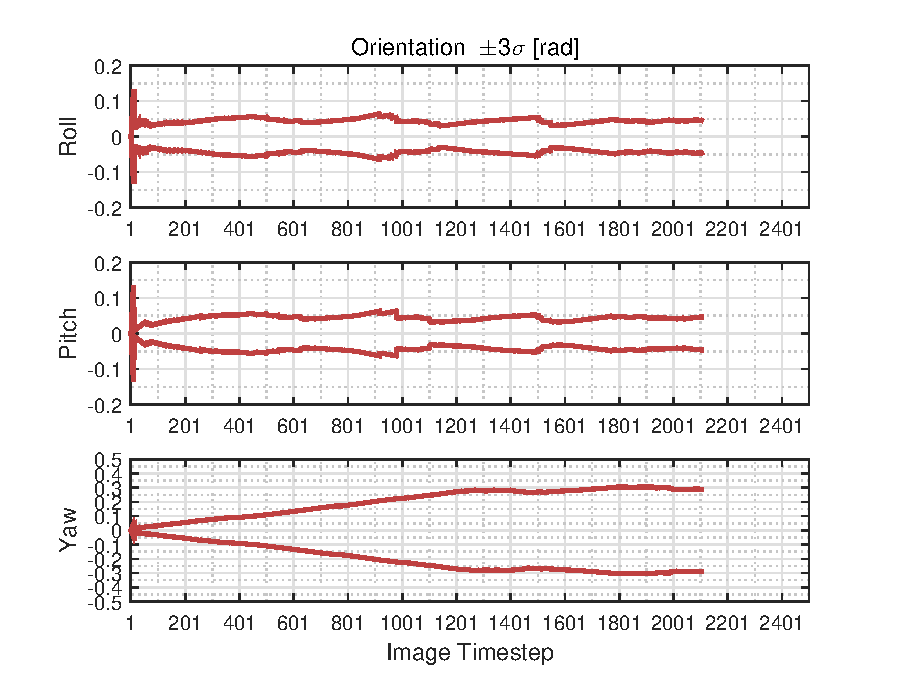
\includegraphics[scale=0.6]{orienation_3sigma.eps}
 	
 	\caption{Estimated orienation $ \pm 3 \sigma $ bounds of Roll, Pitch and Yaw  }
 	\label{figurelabel}
 \end{figure}

The results shown in Fig.8 show the error and $ \pm 3 \sigma $ bounds corresponding to orientation estimate. The plots reveal that the error remains bounded by $ \pm 3 \sigma $ , meaning that the filter is consistent. And the proposed estimator has correct observability properties for VINS.  Roll and pitch are observable, the error bounds do not increase indefinitely.In contrast, those for the position and yaw do continuously increase because they are not observable \cite{kelly2011visual}.



 
 

In Fig.9, IMU biases are estimated. We can see the gyroscope biases exhibit a better convergence than the accelerometer biases. This result may come frome the more direct link of rotational rates to visual errors.
 


\begin{figure}[thpb]
	\centering
	
	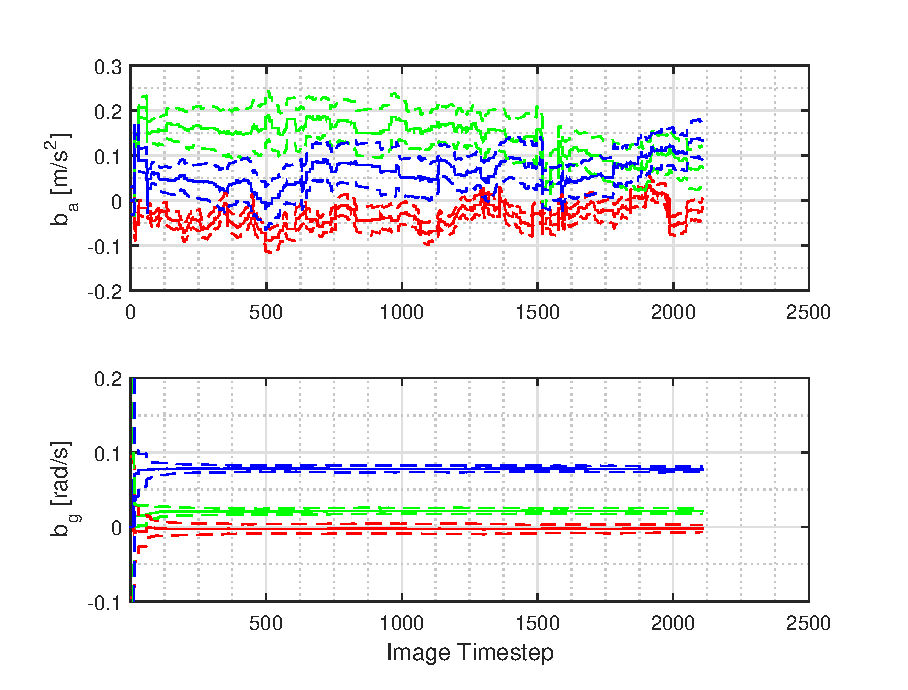
\includegraphics[scale=0.6]{bias.eps}
	
	\caption{Estimated IMU biases with their . Top: accelerometer biases(red:x, green:y, blue:z). Bottom: gyroscope biases(red:x, green:y, blue:z).}
	\label{figurelabel}
\end{figure}

\subsection{Pose Estimation in Dense Probabilistic Mapping}



 VIO is usually used to guide MAVs or other mobile robots moving in either global or local map in navigation task, e.g path planning and obstacle avoidance. These mapping processes require accurate pose estimation. In this section, we integrate the depth perception aligned with the poses estimated by our depth enhanced VIO algorithm to build a dense probabilistic map.


We use LibELAS\cite{geiger2010efficient} to calculate the disparity map. And probabilistic mapping framework OctoMap\cite{hornung2013octomap} is used to fuse multiple meaeurements for space occupancy estimation.



 Fig.10  shows the OctoMap built on $ V2\_02\_medium$ dataset. Different color encodes  variation of hieght. From the top view, although suffered from  depth measurement noise, it can still clearly be seen that the dense map nicely fit the shape of the room and objects on the  ground. This result  validates the precision of our pose estimate method indirectly.





\section{CONCLUSIONS}
In this paper, we have presented a depth enhanced   visual-inertial odometry system based on MSCKF. By integrating visual feature and depth information ,if availible, a 3D meaurement model of landmark position  is derivated, which reduces the estimation uncertainty.  Combining 2D and 3D measuements results in  more   accurate estimation of landmark positon. MSCKF update model is modified to gain compatibility of 2D and 3D measuerment.
\begin{figure}[thpb]
	\centering
	
	\includegraphics[scale=0.81]{octomap1.jpg}
	
	\caption{Top view of OctoMap built on $ V2\_02\_medium$ dataset. Depth measurments are inserted into OctoMap depend on sensor rig poses estimated by the proposed method.}
	\label{figurelabel}
\end{figure}
Experiments under datasets recorded in different scenarios underline the robustness of the proposed method on pose estimate. Compared to mono-MSCKF and other popular open-source method, the proposed gets competitive accuracy. The accuracy  has also been verified by using the system in a probabilistic mapping task.



\addtolength{\textheight}{-12cm}   % This command serves to balance the column lengths
                                  % on the last page of the document manually. It shortens
                                  % the textheight of the last page by a suitable amount.
                                  % This command does not take effect until the next page
                                  % so it should come on the page before the last. Make
                                  % sure that you do not shorten the textheight too much.

%%%%%%%%%%%%%%%%%%%%%%%%%%%%%%%%%%%%%%%%%%%%%%%%%%%%%%%%%%%%%%%%%%%%%%%%%%%%%%%%



%%%%%%%%%%%%%%%%%%%%%%%%%%%%%%%%%%%%%%%%%%%%%%%%%%%%%%%%%%%%%%%%%%%%%%%%%%%%%%%%







%%%%%%%%%%%%%%%%%%%%%%%%%%%%%%%%%%%%%%%%%%%%%%%%%%%%%%%%%%%%%%%%%%%%%%%%%%%%%%%%




\bibliographystyle{IEEEtran}
\bibliography{iros}




\end{document}
